%No editar amenos que el titulo no encaje bien

\begin{titlepage}
\begin{tikzpicture}[remember picture, overlay]
    % Fondo blanco 
    \fill[white] (current page.north west) rectangle ([xshift=9.5cm]current page.south west);
    
    % Franja amarilla vertical
    \fill[ustaAmarillo] ([xshift=13cm]current page.north west) rectangle ([xshift=13.28cm]current page.south west);
    
    % Fondo azul 
    \fill[ustaAzul] ([xshift=13.28cm]current page.north west) rectangle (current page.south east);
    
    % Año en la esquina superior derecha  
    \node[text=white, font=\fontsize{48}{58}\selectfont] at ([xshift=-4.56cm, yshift=-3cm]current page.north east) {\proyectoAnio};

    
    % --- BARRA NEGRA Y TÍTULO ---
    
    % 1. Barra negra más alta (de -7cm a -13cm para dar espacio)
    \fill[black] ([yshift=-7.5cm]current page.north west) rectangle ([xshift=19.5cm, yshift=-12.5cm]current page.north west);
    
    % 2. Título ajustado
    \node[
    text=white, 
    font=\fontsize{20}{24}\selectfont\bfseries, % Añadí negrita (\bfseries) para que se vea mejor
    anchor=center,       % Anclado al centro
    text width=18cm,     % ESTO ES CLAVE: Fuerza al texto a romperse en líneas
    align=center         % Centra el texto dentro del bloque
    ] at ([xshift=9.75cm, yshift=-10cm]current page.north west) % Coordenada: Mitad de ancho (19.5/2) y Mitad de altura (entre -7 y -13)
    {DESARROLLO DE UNA APLICACIÓN WEB PARA LA GESTIÓN DE COMANDAS EN RESTAURANTES PYME CON ENCRIPTACIÓN Y AUTENTICACIÓN DE BAJO COSTO};
    
    % Imagen  
     \node[anchor=west] at ([xshift=8.39cm, yshift=-4cm]current page.west) {
        % Ajusta el ancho (width) para que quepa en la zona blanca (< 8cm)
        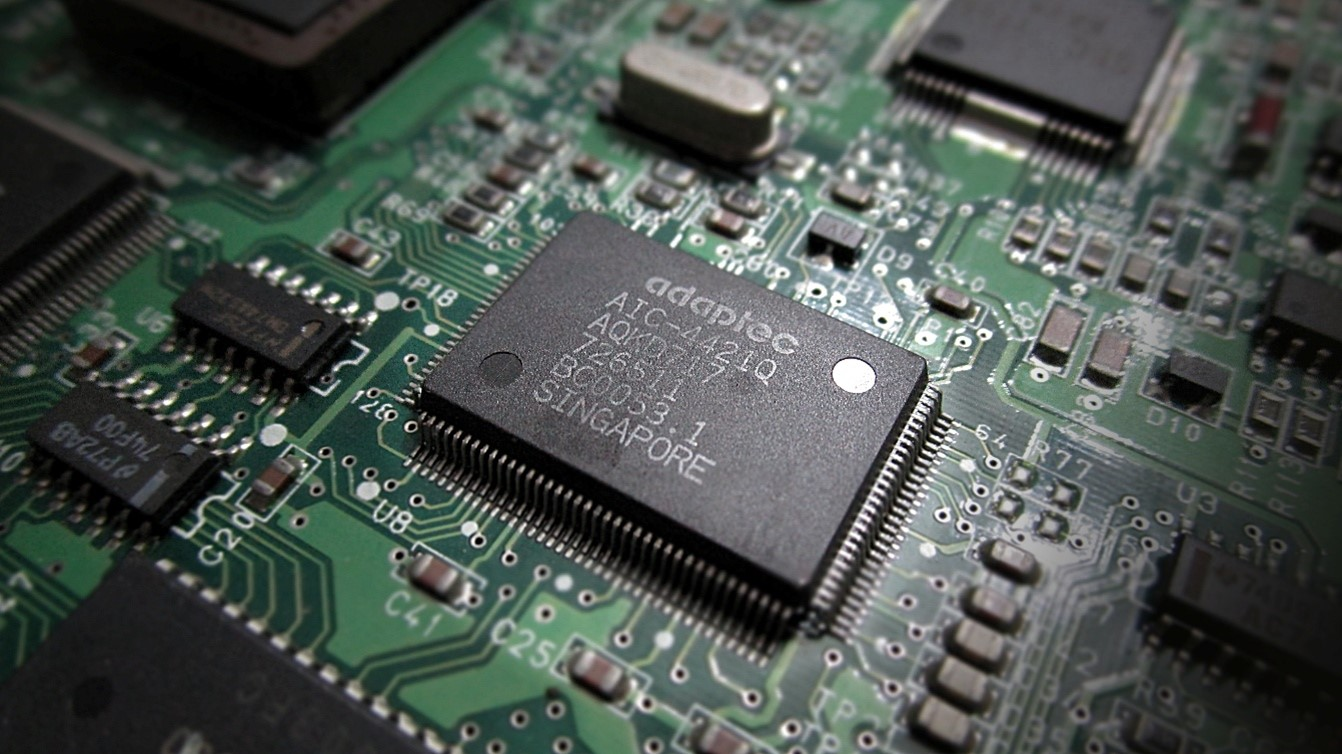
\includegraphics[width=13cm]{imagenes/pcb.jpg} 
    };
    
    % fecha
    \node[text=white, font=\fontsize{11}{13}\selectfont\normalfont, align=right, anchor=south east] 
        at ([xshift=-0.5cm, yshift=2.5cm]current page.south east) {
        \estudianteUno \\        
        Universidad Santo Tomás\\[0.3cm]
        \proyectoFechaCompleta
    };    
   
\end{tikzpicture}
\end{titlepage}
